\newday{11 March 2024}
	
	\action{
		Finally got the output fluxes from the unnormalized mode coefficients
	}
	
	\rule{0.5\textwidth}{0.5pt}\\

	{\large \textbf{EXPERIMENT PSFRecontructorFC10000-1}}\\
	
	{\normalsize HYPERPARAMETERS:}
	\begin{lstlisting}
	*ARCHITECTURE HYPERPARAMETERS:
		-Fully Connected
		-Input shape: 19
		-Output shape: 32768
		-Hidden layers: [256, 256, 256]
		-Regularizer: None
		-Hidden Layers Activation: relu
		-Output Layer Activation: linear
		-Batch Normalization: False
		-Dropout: False, 0.2
	
	*COMPILATION HYPERPARAMETERS:
		-Optimizer: ADAM lr=0.001, beta_1=0.9, beta_2=0.999
		-Loss Function: MSE
		-Metric: MSE
	
	*TRAINING HYPERPARAMETERS:
		-Epochs: 100
		-Batch size: 64
		-Callbacks: 
			-ReduceLROnPlateau: MSE 10 x0.1
			-Early Stop: MSE 25
	\end{lstlisting}
	
	{\normalsize VISUALIZATION:}
	\begin{lstlisting}
    *RESULTS:
        -Train MSE: 0.017938978970050812
        -Validation MSE: 0.055591899901628494
	\end{lstlisting}
	
	\begin{figure*}[ht!]
		\subfloat[Training Evolution]{%
		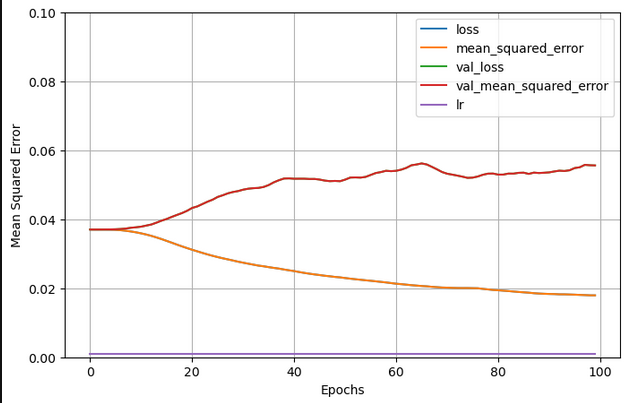
\includegraphics[ width=0.31\textwidth]{psf-PSFRecontructorFC10000-1-evolution.png}}
		\hspace{\fill}
		\subfloat[Validation datapoint]{%
		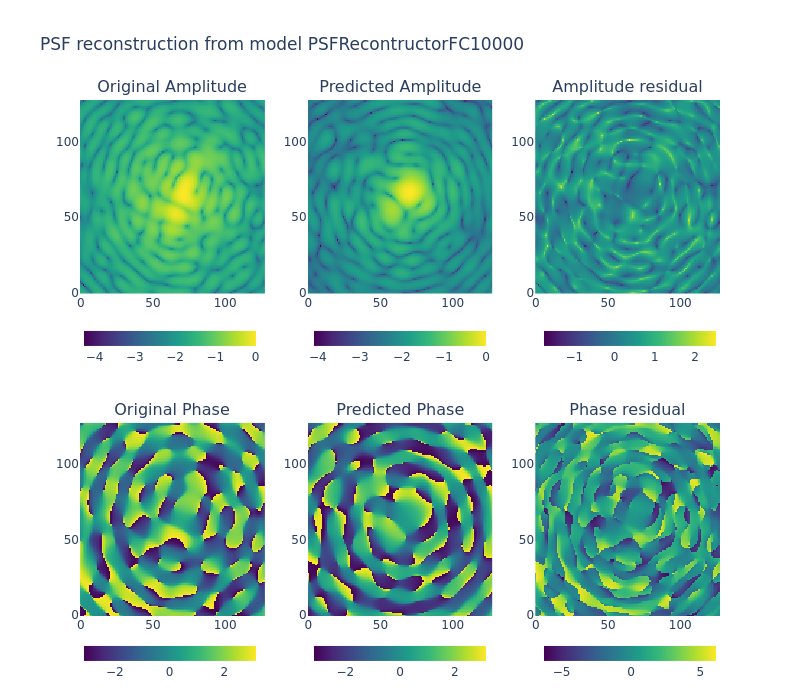
\includegraphics[ width=0.31\textwidth]{psf-PSFRecontructorFC10000-1-val.png}}
		\hspace{\fill}	
		\subfloat[Train datapoint]{%
		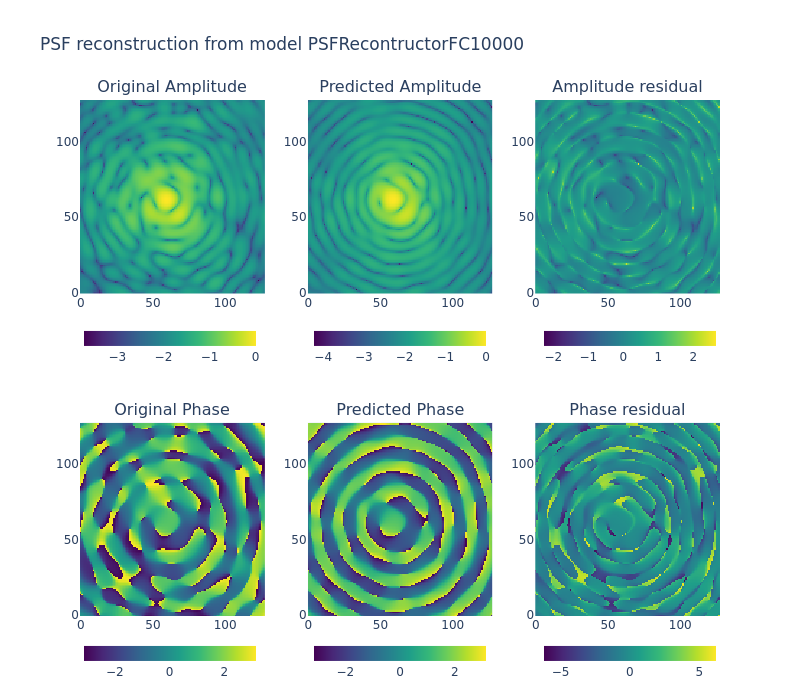
\includegraphics[ width=0.31\textwidth]{psf-PSFRecontructorFC10000-1-train.png}}\\
		\caption{Results of training the model PSFRecontructorFC10000-1}
	\end{figure*}
	
\FloatBarrier	
\rule{0.5\textwidth}{0.5pt}\\
	\rule{0.5\textwidth}{0.5pt}\\

	{\large \textbf{EXPERIMENT PSFRecontructorFC30000-1}}\\
	
	{\normalsize HYPERPARAMETERS:}
	\begin{lstlisting}
	*ARCHITECTURE HYPERPARAMETERS:
		-Fully Connected
		-Input shape: 19
		-Output shape: 32768
		-Hidden layers: [256, 256, 256]
		-Regularizer: None
		-Hidden Layers Activation: relu
		-Output Layer Activation: linear
		-Batch Normalization: False
		-Dropout: False, 0.2
	
	*COMPILATION HYPERPARAMETERS:
		-Optimizer: ADAM lr=0.001, beta_1=0.9, beta_2=0.999
		-Loss Function: MSE
		-Metric: MSE
	
	*TRAINING HYPERPARAMETERS:
		-Epochs: 100
		-Batch size: 64
		-Callbacks: 
			-ReduceLROnPlateau: MSE 10 x0.1
			-Early Stop: MSE 25
	\end{lstlisting}
	
	{\normalsize VISUALIZATION:}
	\begin{lstlisting}
    *RESULTS:
        -Train MSE: 0.03696389123797417
        -Validation MSE: 0.03704820200800896
	\end{lstlisting}
	
	\begin{figure*}[ht!]
		\subfloat[Training Evolution]{%
		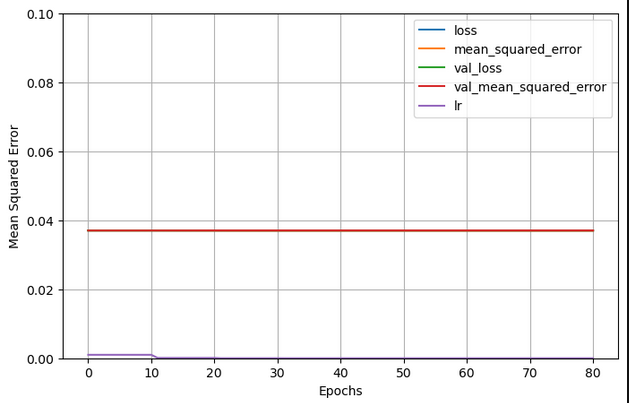
\includegraphics[ width=0.31\textwidth]{psf-PSFRecontructorFC30000-1-evolution.png}}
		\hspace{\fill}
		\subfloat[Validation datapoint]{%
		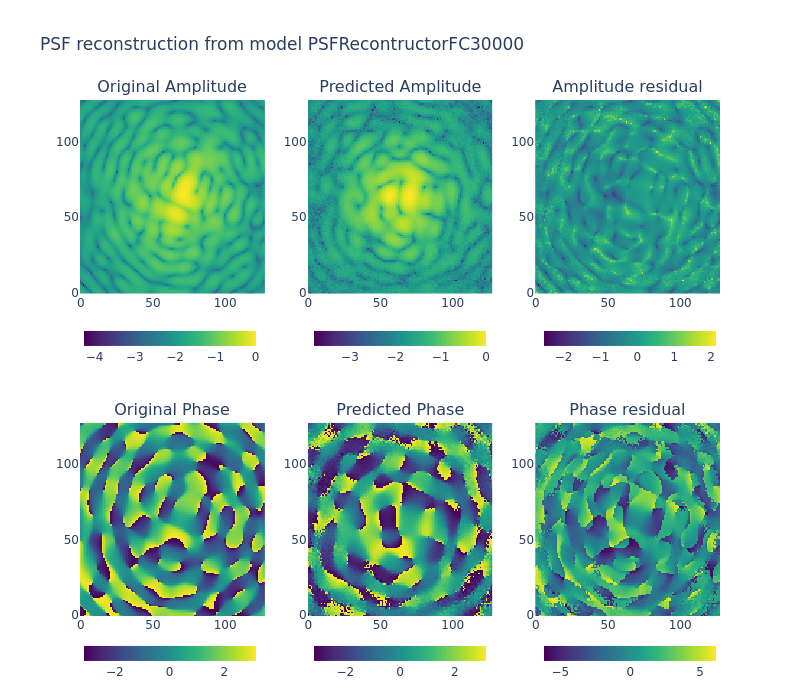
\includegraphics[ width=0.31\textwidth]{psf-PSFRecontructorFC30000-1-val.png}}
		\hspace{\fill}	
		\subfloat[Train datapoint]{%
		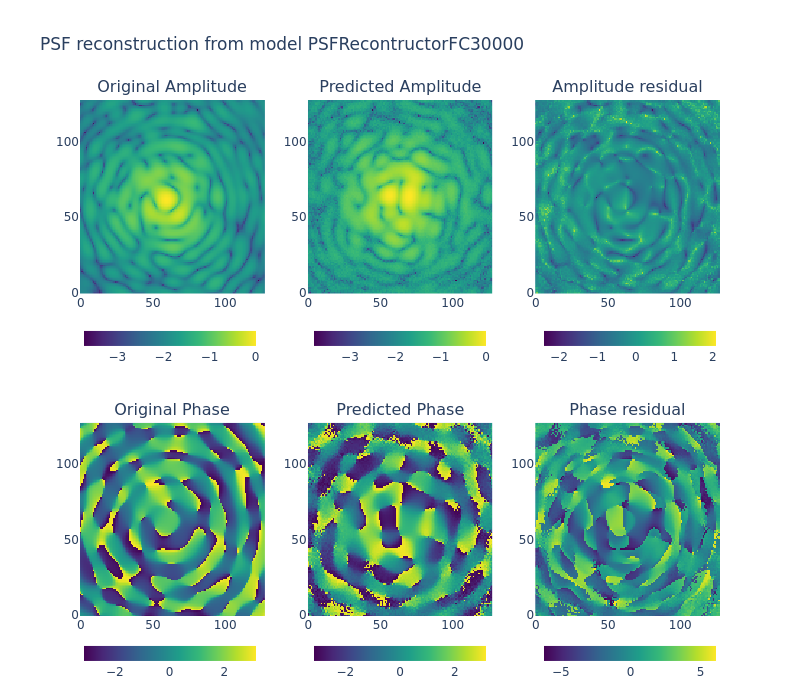
\includegraphics[ width=0.31\textwidth]{psf-PSFRecontructorFC30000-1-train.png}}\\
		\caption{Results of training the model PSFRecontructorFC30000-1}
	\end{figure*}
	
\FloatBarrier	
\rule{0.5\textwidth}{0.5pt}\\
	
	\action{
		Again, flatline, and same output for any input. I will try with all the train dataset and then start using different batch sizes, see how this works
	}
	
	\rule{0.5\textwidth}{0.5pt}\\

	{\large \textbf{EXPERIMENT PSFRecontructorFC70000-1}}\\
	
	{\normalsize HYPERPARAMETERS:}
	\begin{lstlisting}
	*ARCHITECTURE HYPERPARAMETERS:
		-Fully Connected
		-Input shape: 19
		-Output shape: 32768
		-Hidden layers: [256, 256, 256]
		-Regularizer: None
		-Hidden Layers Activation: relu
		-Output Layer Activation: linear
		-Batch Normalization: False
		-Dropout: False, 0.2
	
	*COMPILATION HYPERPARAMETERS:
		-Optimizer: ADAM lr=0.001, beta_1=0.9, beta_2=0.999
		-Loss Function: MSE
		-Metric: MSE
	
	*TRAINING HYPERPARAMETERS:
		-Epochs: 100
		-Batch size: 64
		-Callbacks: 
			-ReduceLROnPlateau: MSE 10 x0.1
			-Early Stop: MSE 25
	\end{lstlisting}
	
	{\normalsize VISUALIZATION:}
	\begin{lstlisting}
    *RESULTS:
        -Train MSE: 0.03700976073741913
        -Validation MSE: 0.0370212197303772
	\end{lstlisting}
	
	\begin{figure*}[ht!]
		\subfloat[Training Evolution]{%
		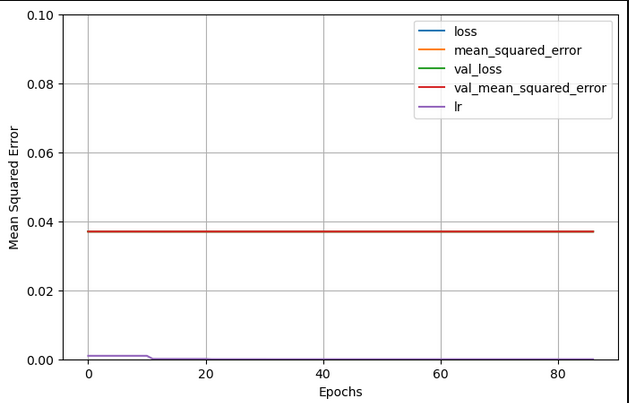
\includegraphics[ width=0.31\textwidth]{psf-PSFRecontructorFC70000-1-evolution.png}}
		\hspace{\fill}
		\subfloat[Validation datapoint]{%
		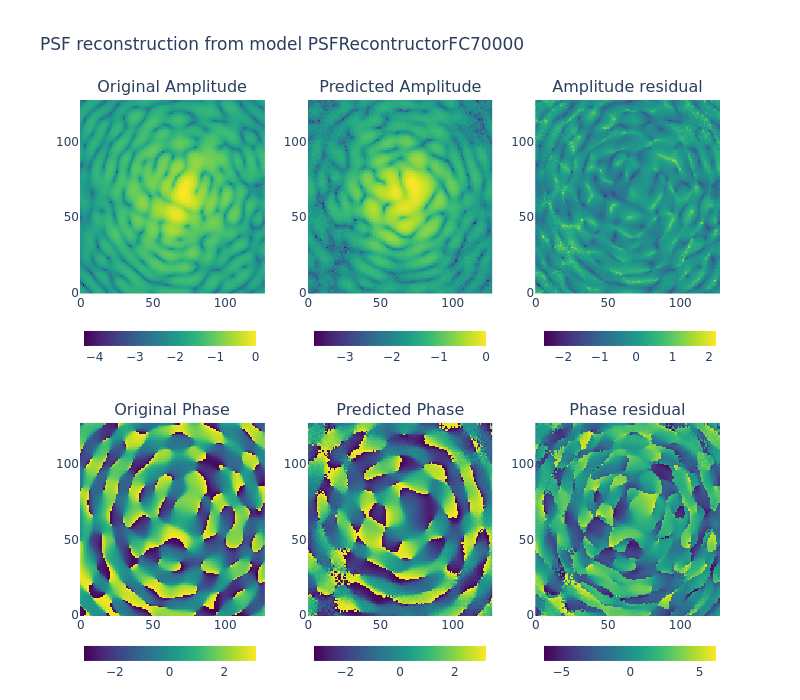
\includegraphics[ width=0.31\textwidth]{psf-PSFRecontructorFC70000-1-val.png}}
		\hspace{\fill}	
		\subfloat[Train datapoint]{%
		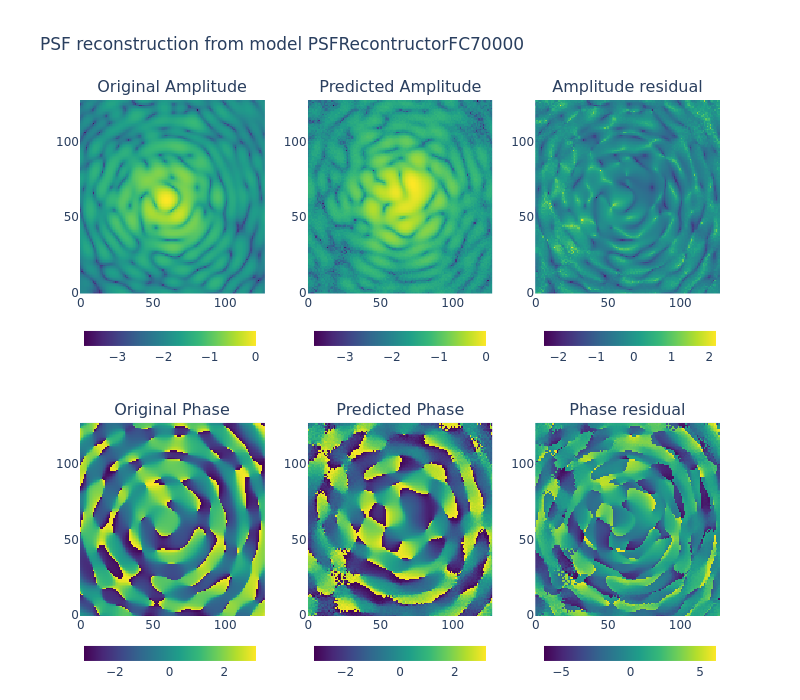
\includegraphics[ width=0.31\textwidth]{psf-PSFRecontructorFC70000-1-train.png}}\\
		\caption{Results of training the model PSFRecontructorFC70000-1}
	\end{figure*}
	
\FloatBarrier	
\rule{0.5\textwidth}{0.5pt}\\
	
	\action{
		Batch size for these experiments is 64, maybe it is too big	, let's try with 32
	}
	
	\rule{0.5\textwidth}{0.5pt}\\

	{\large \textbf{EXPERIMENT PSFRecontructorFC10000-32-1}}\\
	
	{\normalsize HYPERPARAMETERS:}
	\begin{lstlisting}
	*ARCHITECTURE HYPERPARAMETERS:
		-Fully Connected
		-Input shape: 19
		-Output shape: 32768
		-Hidden layers: [256, 256, 256]
		-Regularizer: None
		-Hidden Layers Activation: relu
		-Output Layer Activation: linear
		-Batch Normalization: False
		-Dropout: False, 0.2
	
	*COMPILATION HYPERPARAMETERS:
		-Optimizer: ADAM lr=0.001, beta_1=0.9, beta_2=0.999
		-Loss Function: MSE
		-Metric: MSE
	
	*TRAINING HYPERPARAMETERS:
		-Epochs: 100
		-Batch size: 32
		-Callbacks: 
			-ReduceLROnPlateau: MSE 10 x0.1
			-Early Stop: MSE 25
	\end{lstlisting}
	
	{\normalsize VISUALIZATION:}
	\begin{lstlisting}
    *RESULTS:
        -Train MSE: 0.03432031720876694
        -Validation MSE: 0.038697339594364166
	\end{lstlisting}
	
	\begin{figure*}[ht!]
		\subfloat[Training Evolution]{%
		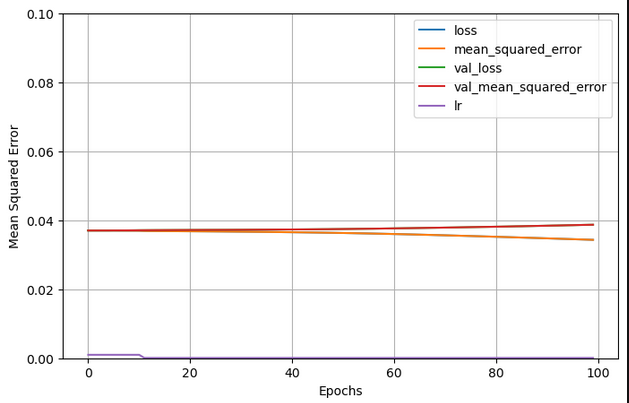
\includegraphics[ width=0.31\textwidth]{psf-PSFRecontructorFC10000-32-1-evolution.png}}
		\hspace{\fill}
		\subfloat[Validation datapoint]{%
		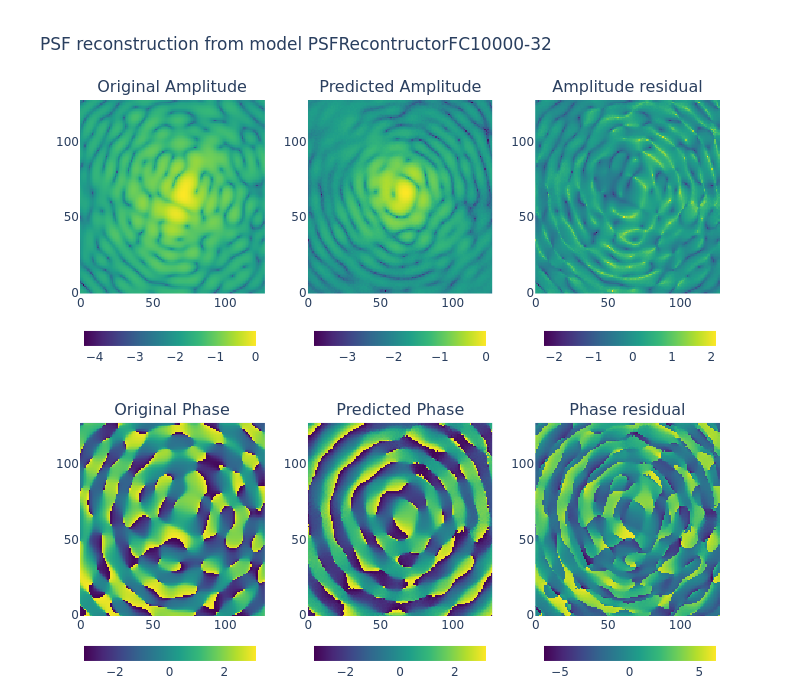
\includegraphics[ width=0.31\textwidth]{psf-PSFRecontructorFC10000-32-1-val.png}}
		\hspace{\fill}	
		\subfloat[Train datapoint]{%
		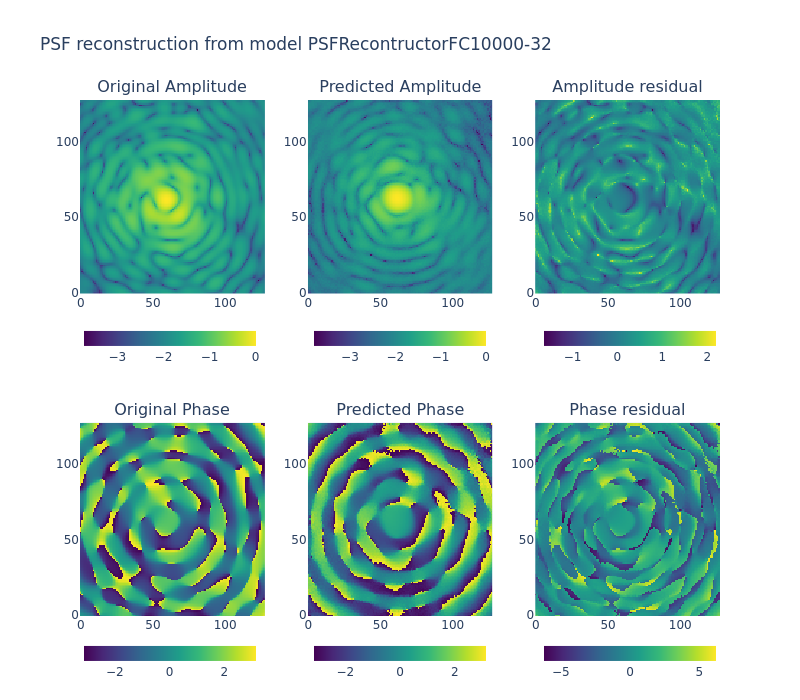
\includegraphics[ width=0.31\textwidth]{psf-PSFRecontructorFC10000-32-1-train.png}}\\
		\caption{Results of training the model PSFRecontructorFC10000-32-1}
	\end{figure*}
	
\FloatBarrier	
\rule{0.5\textwidth}{0.5pt}\\
	
	\action{
		Interesting, slower convergence but less overfitting	
	}
	
	\rule{0.5\textwidth}{0.5pt}\\

	{\large \textbf{EXPERIMENT PSFRecontructorFC30000-32-1}}\\
	
	{\normalsize HYPERPARAMETERS:}
	\begin{lstlisting}
	*ARCHITECTURE HYPERPARAMETERS:
		-Fully Connected
		-Input shape: 19
		-Output shape: 32768
		-Hidden layers: [256, 256, 256]
		-Regularizer: None
		-Hidden Layers Activation: relu
		-Output Layer Activation: linear
		-Batch Normalization: False
		-Dropout: False, 0.2
	
	*COMPILATION HYPERPARAMETERS:
		-Optimizer: ADAM lr=0.001, beta_1=0.9, beta_2=0.999
		-Loss Function: MSE
		-Metric: MSE
	
	*TRAINING HYPERPARAMETERS:
		-Epochs: 100
		-Batch size: 32
		-Callbacks: 
			-ReduceLROnPlateau: MSE 10 x0.1
			-Early Stop: MSE 25
	\end{lstlisting}
	
	{\normalsize VISUALIZATION:}
	\begin{lstlisting}
    *RESULTS:
        -Train MSE: 0.03701305016875267
        -Validation MSE: 0.03701600059866905
	\end{lstlisting}
	
	\begin{figure*}[ht!]
		\subfloat[Training Evolution]{%
		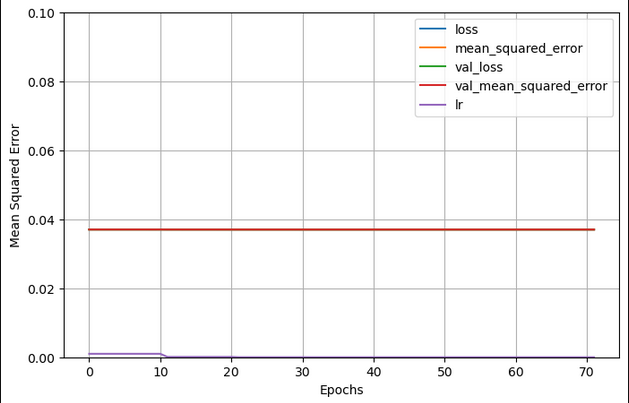
\includegraphics[ width=0.31\textwidth]{psf-PSFRecontructorFC30000-32-1-evolution.png}}
		\hspace{\fill}
		\subfloat[Validation datapoint]{%
		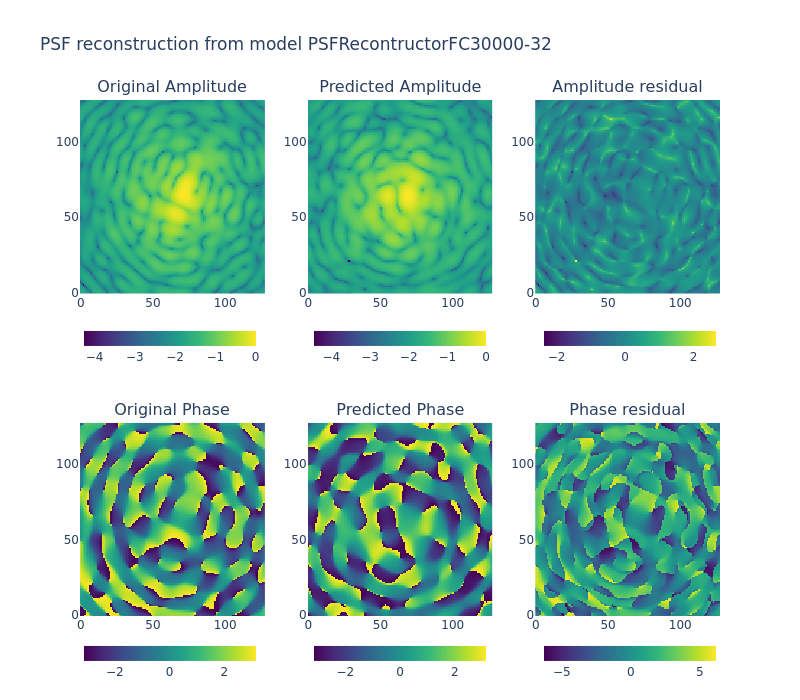
\includegraphics[ width=0.31\textwidth]{psf-PSFRecontructorFC30000-32-1-val.png}}
		\hspace{\fill}	
		\subfloat[Train datapoint]{%
		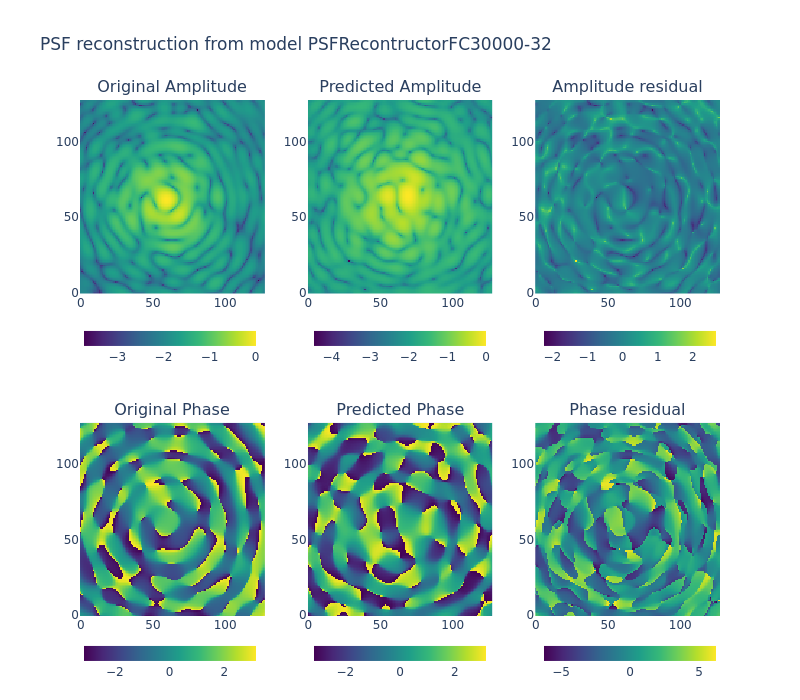
\includegraphics[ width=0.31\textwidth]{psf-PSFRecontructorFC30000-32-1-train.png}}\\
		\caption{Results of training the model PSFRecontructorFC30000-32-1}
	\end{figure*}
	
\FloatBarrier	
\rule{0.5\textwidth}{0.5pt}\\
	\rule{0.5\textwidth}{0.5pt}\\

	{\large \textbf{EXPERIMENT PSFRecontructorFC70000-32-1}}\\
	
	{\normalsize HYPERPARAMETERS:}
	\begin{lstlisting}
	*ARCHITECTURE HYPERPARAMETERS:
		-Fully Connected
		-Input shape: 19
		-Output shape: 32768
		-Hidden layers: [256, 256, 256]
		-Regularizer: None
		-Hidden Layers Activation: relu
		-Output Layer Activation: linear
		-Batch Normalization: False
		-Dropout: False, 0.2
	
	*COMPILATION HYPERPARAMETERS:
		-Optimizer: ADAM lr=0.001, beta_1=0.9, beta_2=0.999
		-Loss Function: MSE
		-Metric: MSE
	
	*TRAINING HYPERPARAMETERS:
		-Epochs: 100
		-Batch size: 32
		-Callbacks: 
			-ReduceLROnPlateau: MSE 10 x0.1
			-Early Stop: MSE 25
	\end{lstlisting}
	
	{\normalsize VISUALIZATION:}
	\begin{lstlisting}
    *RESULTS:
        -Train MSE: 0.03701675683259964
        -Validation MSE: 0.037016723304986954
	\end{lstlisting}
	
	\begin{figure*}[ht!]
		\subfloat[Training Evolution]{%
		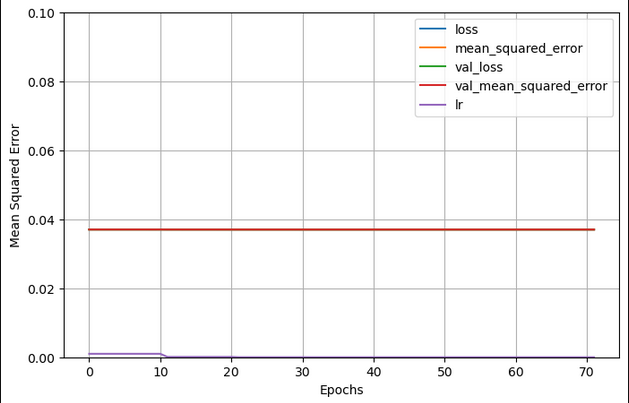
\includegraphics[ width=0.31\textwidth]{psf-PSFRecontructorFC30000-32-1-evolution.png}}
		\hspace{\fill}
		\subfloat[Validation datapoint]{%
		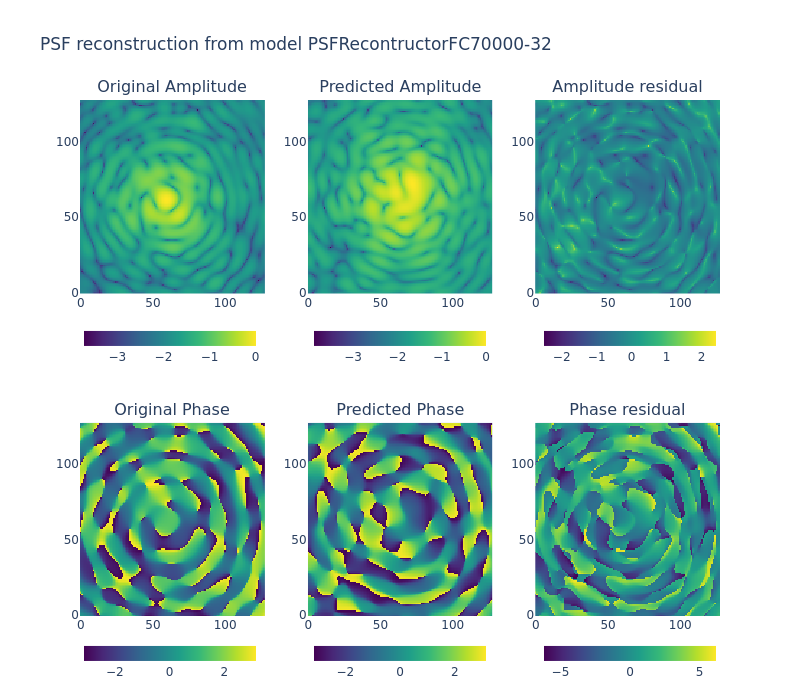
\includegraphics[ width=0.31\textwidth]{psf-PSFRecontructorFC70000-32-1-val.png}}
		\hspace{\fill}	
		\subfloat[Train datapoint]{%
		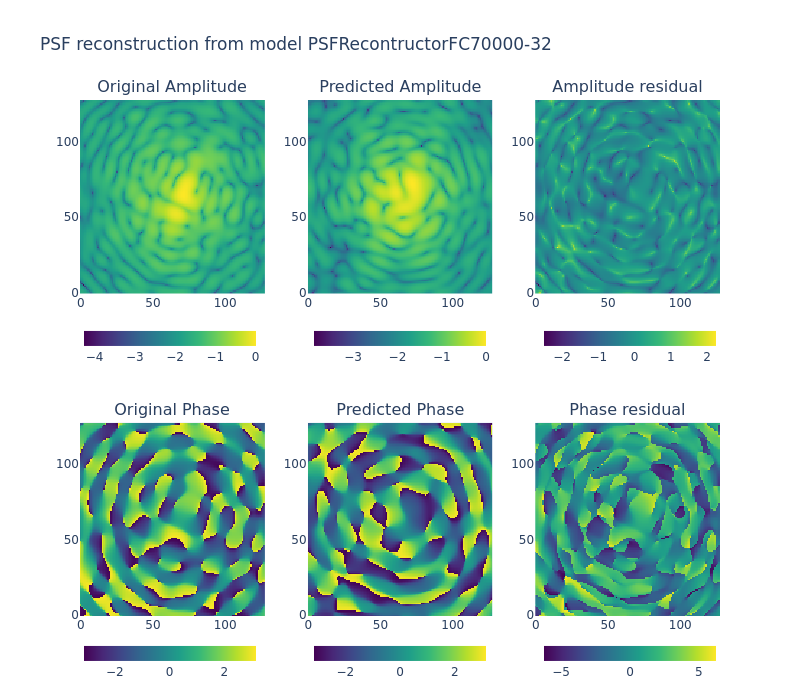
\includegraphics[ width=0.31\textwidth]{psf-PSFRecontructorFC70000-32-1-train.png}}\\
		\caption{Results of training the model PSFRecontructorFC70000-32-1}
	\end{figure*}
	
\FloatBarrier	
\rule{0.5\textwidth}{0.5pt}\\
	
	\action{
		So no good results, what I saw is that the lower the batch size, the longer it takes to coverge. Options now are:
		\begin{itemize}
			\item Bigger NN
			\item Bigger Batch size
			\item Longer training
		\end{itemize}
		
		I will start with 10000 datapoints and a bigger NN		
	}
	
	\rule{0.5\textwidth}{0.5pt}\\

	{\large \textbf{EXPERIMENT PSFRecontructorBigFC10000-32-1}}\\
	
	{\normalsize HYPERPARAMETERS:}
	\begin{lstlisting}	
	*ARCHITECTURE HYPERPARAMETERS:
		-Fully Connected
		-Input shape: 19
		-Output shape: 32768
		-Hidden layers: [256, 256, 256, 256, 256, 256]
		-Regularizer: None
		-Hidden Layers Activation: relu
		-Output Layer Activation: linear
		-Batch Normalization: False
		-Dropout: False, 0.2
	
	*COMPILATION HYPERPARAMETERS:
		-Optimizer: ADAM lr=0.001, beta_1=0.9, beta_2=0.999
		-Loss Function: MSE
		-Metric: MSE
	
	*TRAINING HYPERPARAMETERS:
		-Epochs: 100
		-Batch size: 32
		-Callbacks: 
			-ReduceLROnPlateau: MSE 20 x0.1
			-Early Stop: MSE 50
	\end{lstlisting}
	
	{\normalsize VISUALIZATION:}
	\begin{lstlisting}
	*RESULTS:
        -Train MSE: 0.012548761442303658
        -Validation MSE: 0.0527174137532711
	\end{lstlisting}
	
	\begin{figure*}[ht!]
		\subfloat[Training Evolution]{%
		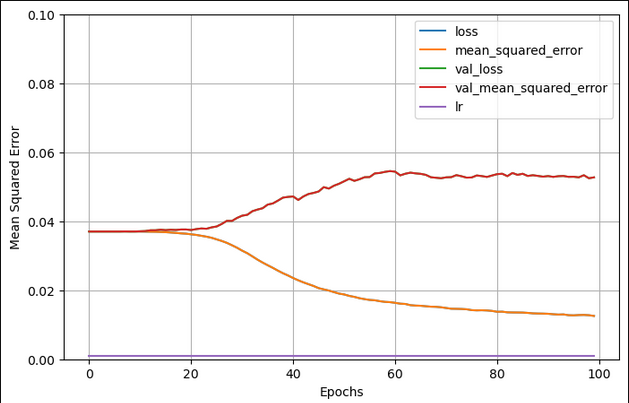
\includegraphics[ width=0.31\textwidth]{psf-PSFRecontructorBigFC10000-32-1-evolution.png}}
		\hspace{\fill}
		\subfloat[Validation example]{%
		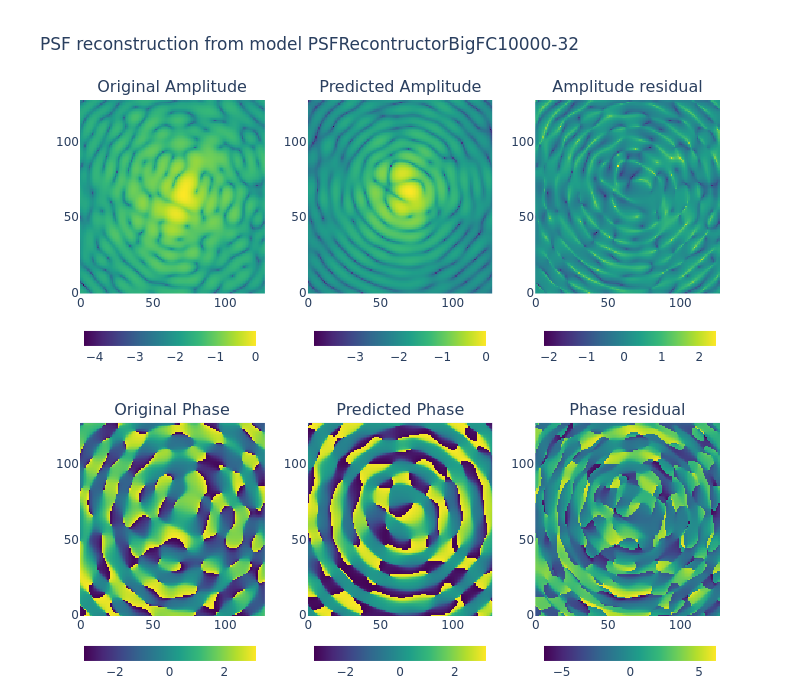
\includegraphics[ width=0.31\textwidth]{psf-PSFRecontructorBigFC10000-32-1-val.png}}
		\hspace{\fill}
		\subfloat[Train example]{%
		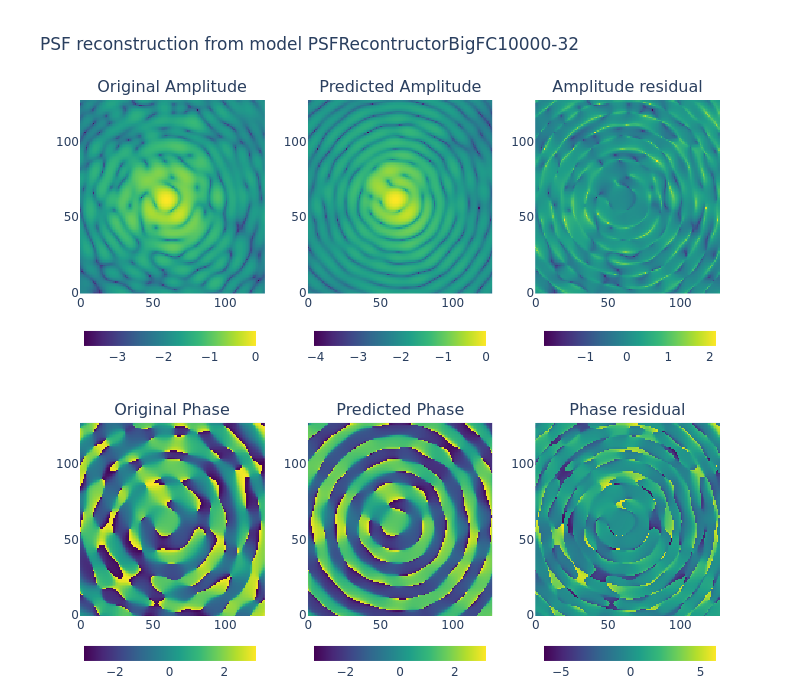
\includegraphics[ width=0.31\textwidth]{psf-PSFRecontructorBigFC10000-32-1-train.png}}\\
		\caption{Results of training the model psf-PSFRecontructorBigFC10000-32-1}
	\end{figure*}
	
\FloatBarrier	
\rule{0.5\textwidth}{0.5pt}\\
	
	\rule{0.5\textwidth}{0.5pt}\\

	{\large \textbf{EXPERIMENT PSFRecontructorBigFC30000-32-1}}\\
	
	{\normalsize HYPERPARAMETERS:}
	\begin{lstlisting}	
	*ARCHITECTURE HYPERPARAMETERS:
		-Fully Connected
		-Input shape: 19
		-Output shape: 32768
		-Hidden layers: [256, 256, 256, 256, 256, 256]
		-Regularizer: None
		-Hidden Layers Activation: relu
		-Output Layer Activation: linear
		-Batch Normalization: False
		-Dropout: False, 0.2
	
	*COMPILATION HYPERPARAMETERS:
		-Optimizer: ADAM lr=0.001, beta_1=0.9, beta_2=0.999
		-Loss Function: MSE
		-Metric: MSE
	
	*TRAINING HYPERPARAMETERS:
		-Epochs: 200
		-Batch size: 32
		-Callbacks: 
			-ReduceLROnPlateau: MSE 20 x0.1
			-Early Stop: MSE 50
	\end{lstlisting}
	
	{\normalsize VISUALIZATION:}
	\begin{lstlisting}
	*RESULTS:
        -Train MSE: 0.025507930666208267
        -Validation MSE: 0.04988955706357956
	\end{lstlisting}
	
	\begin{figure*}[ht!]
		\subfloat[Training Evolution]{%
		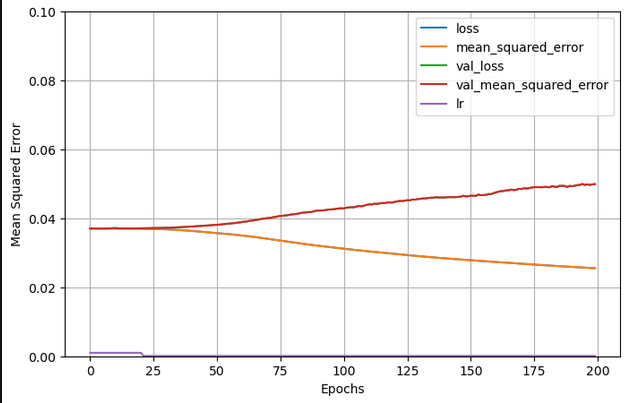
\includegraphics[ width=0.31\textwidth]{psf-PSFRecontructorBigFC30000-32-1-evolution.png}}
		\hspace{\fill}
		\subfloat[Validation example]{%
		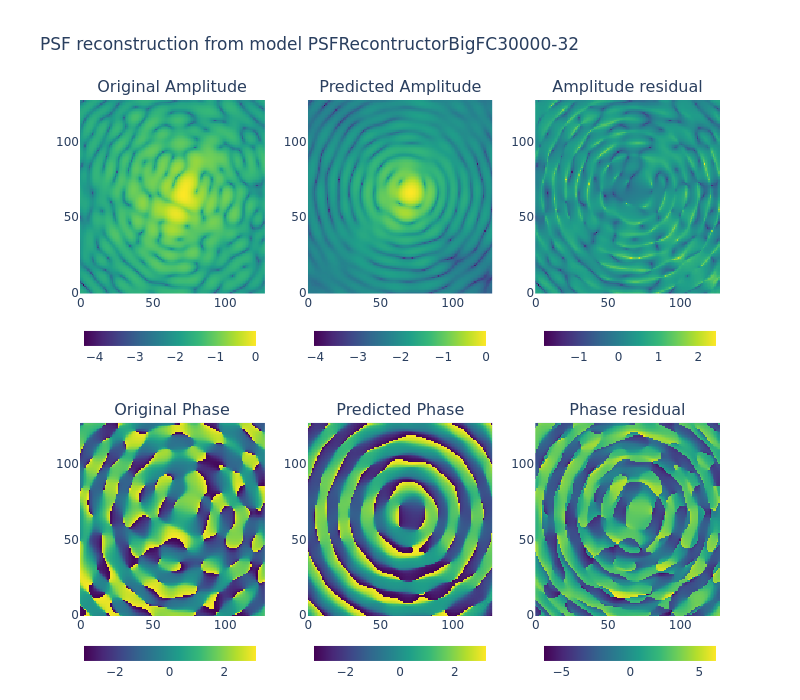
\includegraphics[ width=0.31\textwidth]{psf-PSFRecontructorBigFC30000-32-1-val.png}}
		\hspace{\fill}
		\subfloat[Train example]{%
		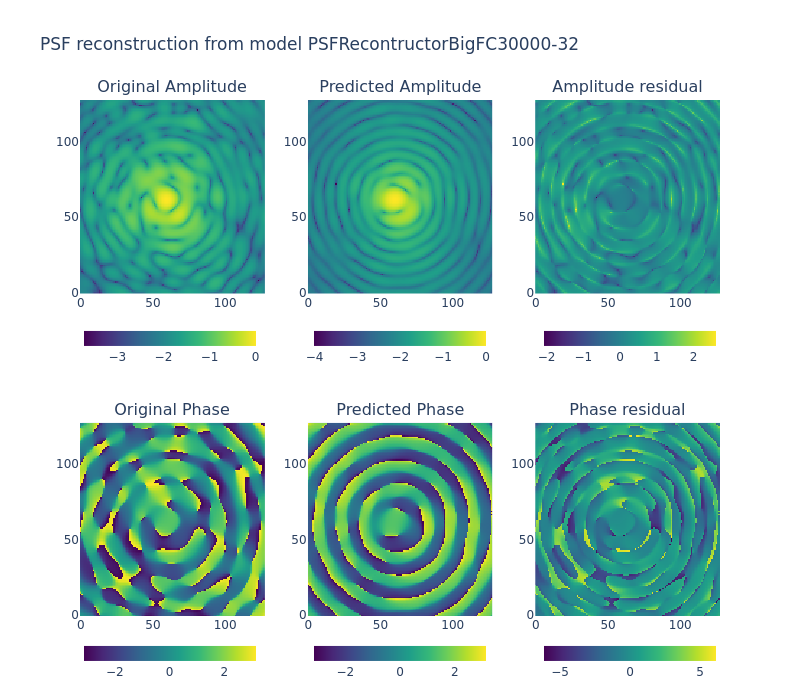
\includegraphics[ width=0.31\textwidth]{psf-PSFRecontructorBigFC30000-32-1-train.png}}\\
		\caption{Results of training the model PSFRecontructorBigFC30000-32-1}
	\end{figure*}
	
\FloatBarrier	
\rule{0.5\textwidth}{0.5pt}\\
	
	\action{
		With respect to the last to experiments, a bigger neural network seems to work better, with more datapoints the learning is delayed a bit, and the overfitting slightly improves, let's check with 70000 datapoints.	
	}
\finishday